
\begin{figure*}[ht]
  \centering 
  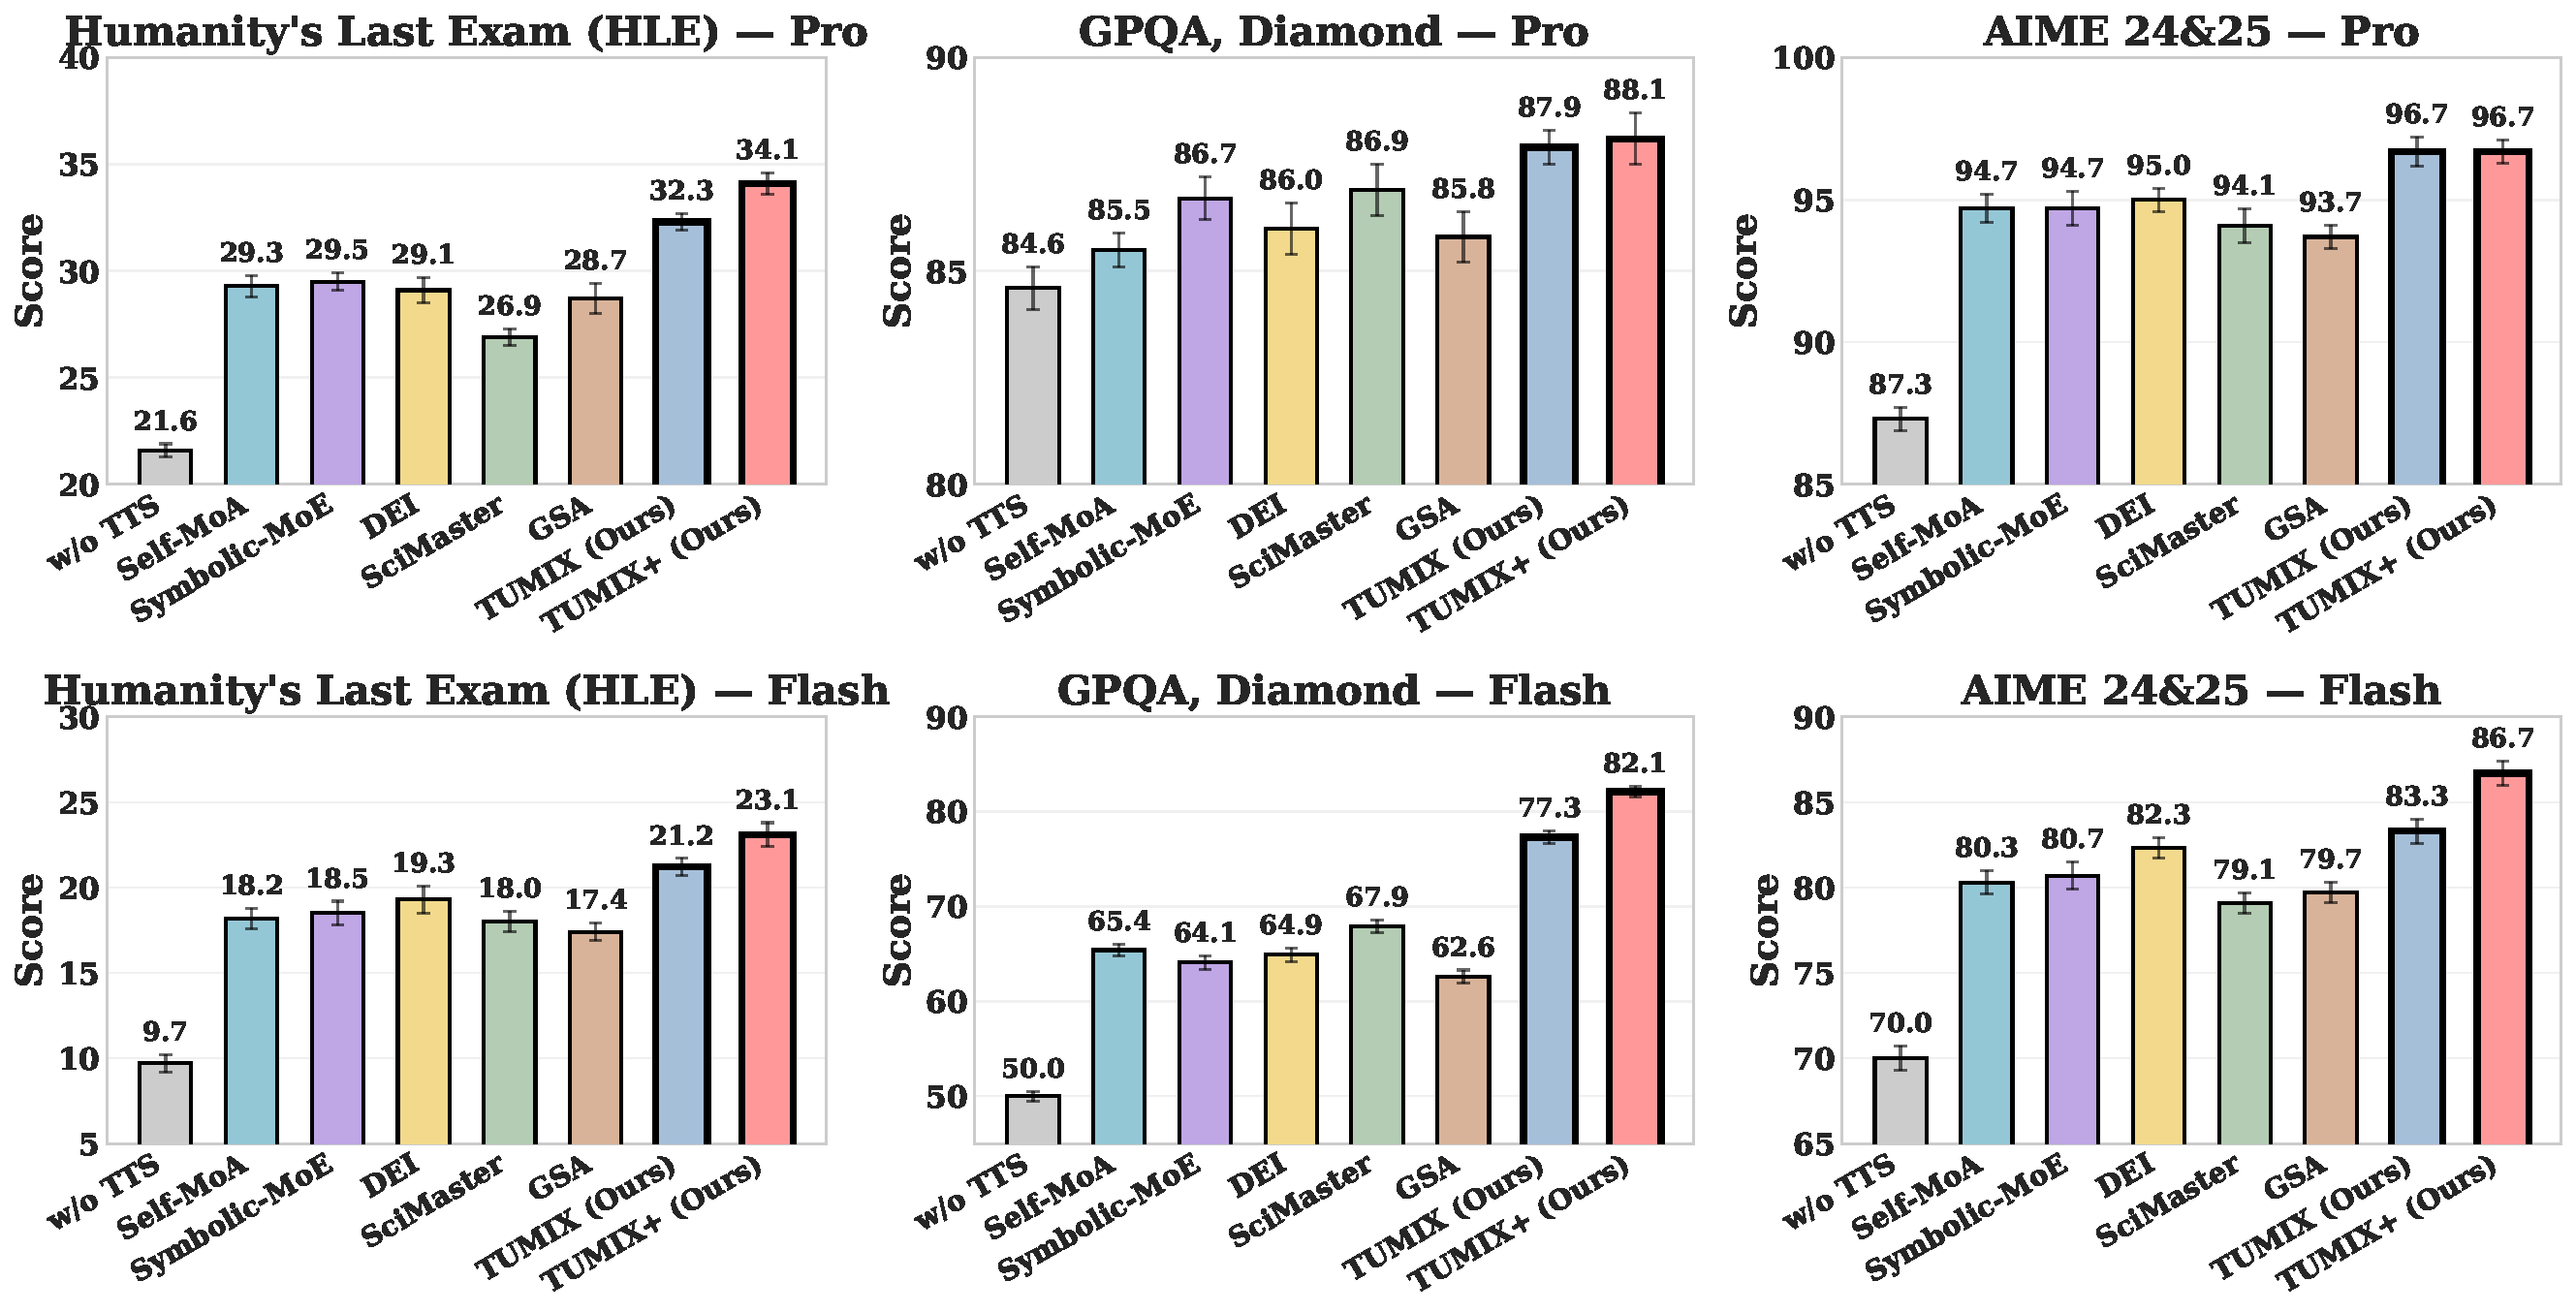
\includegraphics[width=0.95\linewidth]{Figures/tumix_benchmarks_2x3.pdf}
   \caption{Comparison of tool-augmented test-time scaling methods on Gemini-2.5-Pro (first row) and Gemini-2.5-Flash (second row) across HLE, GPQA, and AIME 24\&25. Except for methods without test-time scaling (\texttt{w/o TTS}) or additional scaling (\texttt{TUMIX+}), all methods in the same subplot use nearly the same number of inferences and tokens. For fair comparison, methods that originally lacked tool use are run with strong tool-augmented agents instead of text-only agents. Each score is the average of three repetitive runs.}
   \label{fig:summary_results}
   \vspace{-12pt}
\end{figure*}

\section{Introduction}
While reinforcement learning-based fine-tuning has greatly improved LLM reasoning~\citep{deepseek-r1}, models still struggle with seemingly simple tasks~\citep{codesteering}. 
Such tasks are often better handled with code~\citep{llm+code=commense-learner,Program-of-thoughts-prompting} or search~\citep{search-r1,Search-O1}. 
Textual reasoning is strong in semantics and commonsense, but weak in precise computation and in accessing or updating the latest knowledge.

A key challenge is fully utilizing the potential capabilities of textual reasoning, coding, and searching when facing distinctive questions with varied characteristics. Most input questions lack explicit cues for the best approach, and the combined text/code/search solution space is large. Frontier LLM-powered products such as ChatGPT, Claude, Gemini, and Grok report using code and search at test time to augment reasoning, but without publishing detailed methods. Recent work~\citep{codesteering} shows that current Code Interpreter implementations in OpenAI models often fail to balance text and code, leaving coding capabilities underused, as shown in Appendix Fig.~\ref{fig:GPT-5-fail}. Moreover, public research still lacks a clear understanding of how to integrate Code Interpreter and Search for improved LLM reasoning.

To better leverage both tool use and LLM self-reasoning, we propose Tool-Use Mixture (\texttt{TUMIX}), a framework that integrates Code Interpreter and Search into LLMs via test-time scaling. \texttt{TUMIX} runs multiple diverse agents in parallel, each with different tool-use strategies. Their outputs are iteratively aggregated and refined across multiple rounds. In each round, every agent generates a new solution by considering both the original question and the previous round’s reasoning and answers from all agents. \texttt{TUMIX} uses diverse agents and tool-augmented reasoning strategies to explore a wide range of possible solutions. The following iterative process encourages diverse reasoning paths and deeper integration. This design is inspired by prior test-time scaling methods such as Mixture-of-Agents (MoA)~\citep{MOA}, which rely on multiple LLMs within a single framework and do not incorporate external tools. In contrast, \texttt{TUMIX} employs a single LLM with both text-only and tool-augmented agent frameworks, making it more generalizable for practical applications. Furthermore, in tool-augmented multi-agent test-time scaling, we find a diverse group of agents outperforms repeated use of the single best agent, a conclusion that differs from MoA~\citep{rethink-MOA}. We later reveal that human pre-designed agent group can be further optimized by querying LLMs to self-design more diverse high-quality agents based on current ones, adding an average 1.2\% improvement without cost increase.

Since questions vary in difficulty, they require different amounts of iterative refinement. We query the LLMs to decide whether to terminate refinement early, while still enforcing a minimum number of rounds to maintain answer quality. This adaptive early-termination strategy reduces inference costs to 49\% of the original two settings (termination in a fixed round number or by majority-vote consistency across rounds), while preserving or even improving performance. The improvement arises because over-refinement rarely changes the final result and can even degrade performance, as correct answers may be mistakenly discarded.

Compared to the model without test-time scaling, \texttt{TUMIX} delivers an average +7.8\% and +17.4\% accuracy gains in benchmarks Humanity’s Last Exam (HLE)~\citep{HLE}, Graduate-Level Google-Proof Q\&A (GPQA, Diamond)~\citep{gpqa}, and American Invitational Mathematics Examination (AIME 24\&25) with base models Gemini-2.5-Pro and Gemini-2.5-Flash, respectively. Under the same inference costs, \texttt{TUMIX} also outperforms existing representative test-time scaling methods such as Self-MoA, Symbolic-MoE, DEI, SciMaster, and GSA, with an average +3.55\% lifting compared to the best performing baselines. Notably, with further scaling, \texttt{TUMIX} raises Gemini-2.5-Pro accuracy on HLE from 21.6\% to 34.1\%, surpassing Gemini-2.5-Pro Deep Research at 26.9\% (32.4\% with higher compute)~\citep{Gemini-2.5-Pro}. Test-time scaling hinges on two stages~\citep{LLM-monkey}: (1) generating diverse candidate solutions and (2) selecting the correct one. For questions with both small answer spaces (e.g., multiple-choice) and large ones, diverse sampling greatly improves coverage. While it achieves high coverage on HLE (among generated answers in the whole round, at least one is correct on $\geq 65\%$ of questions), accuracy plateaus at about 34\% because LLMs struggle to identify the correct answer among noisy candidates. We identify and explore four key factors: agent quality, agent diversity, refinement termination, and answer selection. Our work makes the following contributions:

1. \textbf{TUMIX: A competitive tool-augmented test-time scaling method.}\quad We propose \texttt{TUMIX}, a novel framework for test-time scaling that integrates tool augmentation. Extensive experiments demonstrate that \texttt{TUMIX} consistently outperforms strong baselines, achieving an average improvement of +3.55\% over the best-performing prior methods.

2. \textbf{Key factors and mechanisms in tool-augmented scaling.}\quad We provide a systematic analysis that distinguishes tool-augmented scaling from traditional test-time scaling:  
\begin{itemize}[left=0pt, nosep]
    \item \textit{Agent diversity and quality outweigh scale alone.} High-temperature sampling increases coverage, but heterogeneous agent strategies yield higher accuracy and lower cost than repeatedly sampling from a single best-performing agent.  
    \item \textit{Tool augmentation boosts performance.} Agent groups equipped with tools such as Code Interpreter and Search achieve superior coverage and accuracy compared to text-only agent groups.
\end{itemize}

3. \textbf{LLMs as agent designers.}\quad We show that prompting LLMs to automatically generate diverse, high-quality agents based on existing ones further improves \texttt{TUMIX}. This yields an additional average accuracy lift of +1.2\%.

4. \textbf{LLM-as-Judge for refinement termination.}\quad We introduce an LLM-based judge to adaptively determine the optimal stopping round in iterative refinement. This prevents excessive refinement, which reduces diversity and can mistakenly discard correct answers. By enforcing a minimum refinement depth and querying the judge for termination, we achieve near-optimal accuracy while reducing inference cost to $\sim$49\% of the original.
